\documentclass[tikz,border=2mm,background=white]{standalone}
\usepackage{tikz}
\usetikzlibrary{arrows.meta,positioning}

\tikzset{
  box/.style={rectangle, draw=black, fill=blue!15, font=\bfseries\large, 
              minimum width=2.5cm, minimum height=1.2cm, align=center},
  solidArrow/.style={->, thick},
  dashedArrow/.style={->, thick, dashed},
  newOp/.style={draw=black, line width=2pt} % fix: add draw
}

\begin{document}
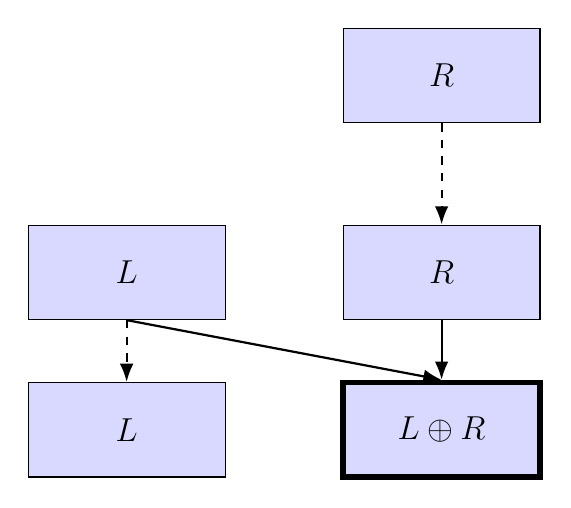
\begin{tikzpicture}[>=Latex]

% Top boxes
\node[box] (Rtop) at (4,0) {$R$};

% Bottom boxes
\node[box] (Lmid) at (0,-2.5) {$L$};
\node[box] (Rmid) at (4,-2.5) {$R$};

% Bottom boxes
\node[box] (Lbot) at (0,-4.5) {$L$};
\node[box,newOp] (Rbot) at (4,-4.5) {$L \oplus R$};

% Solid arrows
\draw[solidArrow] (Lmid.south) -- (Rbot.north);
\draw[solidArrow] (Rmid.south) -- (Rbot.north);

% Dashed arrow
\draw[dashedArrow] (Lmid.south) -- (Lbot.north);
\draw[dashedArrow] (Rtop.south) -- (Rmid.north);

\end{tikzpicture}
\end{document}
